\section{Selección de data (activos, frecuencia)}

Los datos para pruebas y experimentos se descargaron desde la plataforma
Dukascopy. Incialmente las pruebas se realizaron con datos a frecuencia de 1
minuto, pero luego se implementó en clase Reader los métodos correspondientes
para manejar la data ticks de forma automática: juntar datos de distintas monedas
(Bid o Ask), hacer un resampling a diferentes frecuencias, normalizar las
monedas dejando siempre la misma base, etc.

Los ticks están compuestos por: \emph{Date}, \emph{Time}, \emph{Ask},
\emph{Bid}, \emph{AskVolume}, \emph{BidVolume}. Por ser datos ticks, el campo
Time es un hora \emph{double}, es decir, tiene asociada una
hora:minutos:segundos, donde segundos es un número no entero. Cabe destacar que
no existe una clara relación entre la aparición de ticks, ya que en algunos
casos aparecen hasta 4 ticks en 1 segundo, mientras que en otros horarios no
aparecen ticks en 90 segundos (dato calculado con la función
check\_min\_frequency de la clase Reader). 

En la figura \ref{fig:eurusd_ticks} se puede apreciar la data ticks del EURUSD,
en una ventana de 30 minutos, donde la curva superior es la correspondiente al
Ask, y la inferior al Bid. En la figura \ref{fig:eurusd_r6s} se muestra la
misma moneda pero con un resample de 6 segundos. El resample se calcula con el
promedio de los ticks en la ventana de 6 segundos, y para el caso que no exista
movimiento en dicho periodo, se rellena con el valor anteior.

\begin{figure}[h!t]
    \begin{center}
        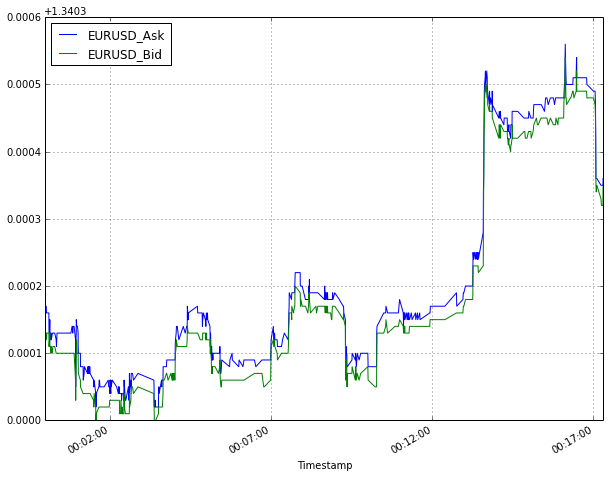
\includegraphics[width=0.6\textwidth]{images/eurusd}
        \caption{Ticks de EURUSD, Ventana de 30 minutos}
        \label{fig:eurusd_ticks}
    \end{center}
\end{figure}

\begin{figure}[h!t]
    \begin{center}
        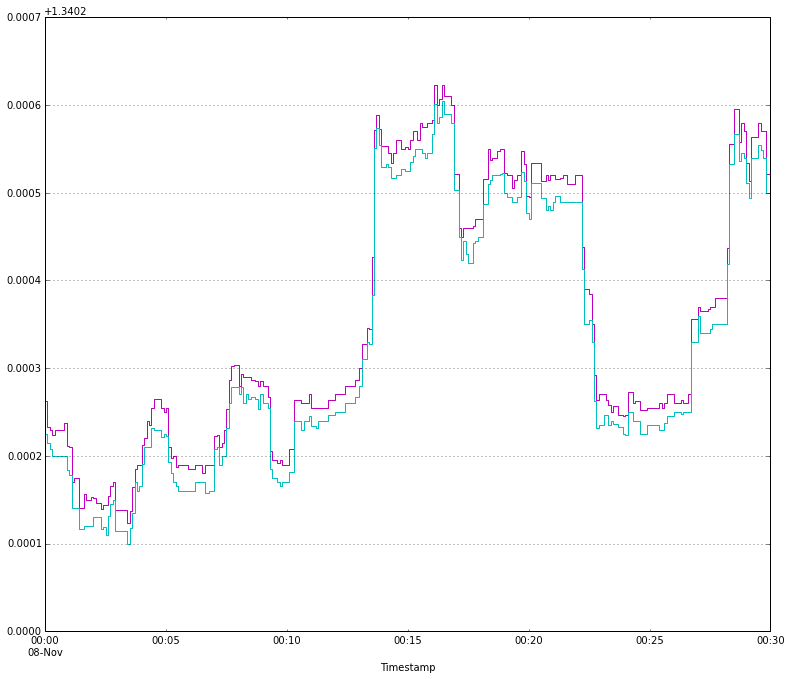
\includegraphics[width=0.6\textwidth]{images/eurusd_6s}
        \caption{Ticks de EURUSD con resample de 6 segundos}
        \label{fig:eurusd_r6s}
    \end{center}
\end{figure}

\section{Parámetros del algoritmo}
Cómo se puede desprender de la formulación matemática de los modelos, hay dos parámetros que deben ser definidos: largo de la ventana (L), cantidad de lags (P). Para ello se usará el criterio de información de Akaike Information Criterion (AIC).

\subsection{Akaike Information Criterion}


\section{MAPE}

\section{Performance}

